% !TEX TS-program = xelatex
% !TEX encoding = UTF-8 Unicode

\documentclass[a4paper,twoside,12pt]{book}
%\usepackage[utf8]{inputenc}
\usepackage{fontspec}
\usepackage{graphicx}
\usepackage[russian]{babel}
\usepackage{hyperref}
%\hypersetup{pdftex,colorlinks=true,allcolors=blue}
\usepackage{hypcap}

\graphicspath{ {Pics/} }

% Times New Roman
\setromanfont[
BoldFont=timesbd.ttf,
ItalicFont=timesi.ttf,
BoldItalicFont=timesbi.ttf,
]{times.ttf}
% Arial
\setsansfont[
BoldFont=arialbd.ttf,
ItalicFont=ariali.ttf,
BoldItalicFont=arialbi.ttf
]{arial.ttf}
% Courier New
\setmonofont[Scale=0.90,
BoldFont=courbd.ttf,
ItalicFont=couri.ttf,
BoldItalicFont=courbi.ttf,
Color={0019D4}
]{cour.ttf}

\begin{document}

\author{Алексей Миронов}
\title{Программирование\\
для АБИС "ИРБИС64"\\
в среде .NET Framework}
\date{Июль 2016}

\frontmatter
\maketitle

\clearpage
\thispagestyle{empty}
	Описаны возможности расширения АБИС "ИРБИС64",
	серверный протокол и фреймворк ManagedIrbis,
	позволяющий создавать приложения произвольной
	сложности на основе "ИРБИС64".
	
	Для автоматизаторов библиотек и программистов,
	создающих решения для "ИРБИС64".

\tableofcontents

\mainmatter
\chapter*{Введение}
\addcontentsline{toc}{chapter}{Введение}
\chaptermark{Введение}

Фреймворк «ManagedIrbis» предназначен для организации программного доступа к ресурсам, находящихся под управлением сервера ИРБИС64, и может использоваться для как для расширения функциональности стандартных АРМ, входящих в поставку АБИС ИРБИС64, так и для создания собственных программных продуктов, совместимых с ИРБИС64.

\section*{Совместимость}

Фреймворк совместим со следующими версиями ИРБИС64:
2004	2005	2006	2007	2008	2009	2010	2011	2012	2013	2014	2015

Совместимость с конкретной версией сервера ИРБИС64 устанавливается по результатам прогона набора стандартных тестов: подключение к серверу, получение служебной информации (версия сервера, количество лицензий и т. д.), чтение записей, форматирование записей, сохранение записей и т. д.

\section*{Инструментарий}

Фреймворк написан на языке C\# в среде Microsoft Visual Studio 2013 для Micorsoft .NET Framework 4.5. Для сборки библиотеки из исходных текстов необходим совместимый инструментарий: Visual Studio 2013 или более новой версии как бесплатной редакции (Express), так и платной (Standard, Profes\-sional и т. д.).

Библиотека должна без модификации успешно собираться средами Mono\-Develop (версия не ниже 4.0) и Sharp\-Develop (версия не ниже 4.4).
Однако всё многообразие альтернативного инструментария не было протестировано авторами (и они не ставили перед собой подобной задачи), и авторы рекомендуют использовать для сборки Visual Studio 2013.

\section*{Системные требования}

Основным системным требованием библиотеки является наличие Microsoft.Net framework 4.5/4.5.1/4.5.2 или совместимой с ним среды исполнения управляемого кода.
Фреймворк должен функционировать в следующем окружении:

\begin{table}[htbp]
	\centering
	\caption{Поддерживаемые окружения}
	\begin{tabular}{ | p{0.4\textwidth} | p{0.4\textwidth} | }
	\hline
	\textbf{Окружение} & 
	\textbf{Функционирование, требования}
	\\
	\hline
	\hline
	Microsoft Windows XP & Не поддерживается \\
	\hline
	Microsoft Windows Vista SP2 & Необходимо установить .Net framework 4.5 \\
	\hline
	Microsoft Windows Server 2003 & Не поддерживается \\
	\hline
	Microsoft Windows 7 SP1 & Необходимо установить .Net framework 4.5 \\
	\hline
	Microsoft Windows Server 2008 SP2/2008 R2 SP1 & Необходимо установить .Net framework 4.5 \\
	\hline
	Microsoft Windows Server 2012/2012 R2 & Предустановлен в операционной системе \\
	\hline
	\end{tabular}
\end{table}

\section*{ManagedIrbis в Интернет}

Исходные коды фреймворка размещены на Git-хостинге github.com по адресу https://github.com/amironov73/arsmagna. Доступ к репозиторию открыт на чтение для всех.
Исполняемые файлы фреймворка опубликованы на сервисе NuGet по адресу

\section*{Лицензия}

Фреймворк распространяется как продукт с открытым исходным кодом. Любой желающий может:

\begin{itemize}
	\item Использовать бинарный релиз библиотеки в своих проектах в неизменном виде – в этом случае требуется лишь указание на авторство библиотеки.
	\item Адаптировать исходный код для собственных нужд и использовать в своих проектах модифицированную версию библиотеки или [модифицированные] фрагменты кода из неё – в этом случае требуется указание на авторство библиотеки и факт модификации её кода.
\end{itemize}

Никаких лицензионных отчислений в вышеперечисленных случаях не требуется. 

\section*{Благодарности}

Авторы выражают благодарность:

\begin{itemize}
	\item \textbf{Ивану Батраку} (СФУ), протестировавшему библиотеку на совместимость со старыми версиями ИРБИС-сервера;
	\item \textbf{Арсению Валентиновичу Шувалову} (Саратовская государственная консерватория им. Л. В. Собинова), выявившему ошибки в библиотеке;
	\item \textbf{Артёму Васильевичу Гончарову} (Научная музыкальная библиотека Санкт-Петер\-бургской Консерватории им. Н. А. Римского-Корсакова), выявившему некоторые досадные ошибки в библиотеке.
\end{itemize}

\section*{Версии и совместимость}

Данное руководство описывает версию 1.3.0.24 библиотеки. Версия библиотеки физически хранится как ресурс VERSION сборки ManagedClient.dll и как статическое свойство Version класса ManagedClient64.

Подробнее о проверке версий см. пункт «Определение версии сервера и клиента».
На данный момент несовместимых версий библиотеки нет, поэтому обновление может осуществляться простым копированием новой сборки поверх старой.
Все будущие несовместимости, если таковые появятся, будут описаны в данном разделе.



\chapter{ИРБИС64-сервер и его окружение}

\begin{description}
	\item[Сервер] это сервер
	\item[Клиент] это клиент
\end{description}

У попа была собака. Он её любил. Она съела кусок мяса. Он её убил. В землю закопал. Надпись написал. У попа была собака. Он её любил. Она съела кусок мяса. Он её убил. В землю закопал. Надпись написал.

У попа была собака. Он её любил. Она съела кусок мяса. Он её убил. В землю закопал. Надпись написал. У попа была собака. Он её любил. Она съела кусок мяса. Он её убил. В землю закопал. Надпись написал. У попа была собака. Он её любил. Она съела кусок мяса. Он её убил. В землю закопал. Надпись написал.

У попа была собака. Он её любил. Она съела кусок мяса. Он её убил. В землю закопал. Надпись написал.

У попа была собака. Он её любил. Она съела кусок мяса. Он её убил. В землю закопал. Надпись написал.

У попа была собака. Он её любил. Она съела кусок мяса. Он её убил. В землю закопал. Надпись написал. У попа была собака. Он её любил. Она съела кусок мяса. Он её убил. В землю закопал. Надпись написал.
\chapter{Протокол ИРБИС64}

У попа была собака. Он её любил. Она съела кусок мяса. Он её убил. В землю закопал. Надпись написал. У попа была собака. Он её любил. Она съела кусок мяса. Он её убил. В землю закопал. Надпись написал.

У попа была собака. Он её любил. Она съела кусок мяса. Он её убил. В землю закопал. Надпись написал. У попа была собака. Он её любил. Она съела кусок мяса. Он её убил. В землю закопал. Надпись написал. У попа была собака. Он её любил. Она съела кусок мяса. Он её убил. В землю закопал. Надпись написал.

У попа была собака. Он её любил. Она съела кусок мяса. Он её убил. В землю закопал. Надпись написал.

У попа была собака. Он её любил. Она съела кусок мяса. Он её убил. В землю закопал. Надпись написал.

У попа была собака. Он её любил. Она съела кусок мяса. Он её убил. В землю закопал. Надпись написал. У попа была собака. Он её любил. Она съела кусок мяса. Он её убил. В землю закопал. Надпись написал.
\chapter{ManagedIrbis. Быстрый старт}

У попа была собака. Он её любил. Она съела кусок мяса. Он её убил. В землю закопал. Надпись написал. У попа была собака. Он её любил. Она съела кусок мяса. Он её убил. В землю закопал. Надпись написал.

У попа была собака. Он её любил. Она съела кусок мяса. Он её убил. В землю закопал. Надпись написал. У попа была собака. Он её любил. Она съела кусок мяса. Он её убил. В землю закопал. Надпись написал. У попа была собака. Он её любил. Она съела кусок мяса. Он её убил. В землю закопал. Надпись написал.

У попа была собака. Он её любил. Она съела кусок мяса. Он её убил. В землю закопал. Надпись написал.

У попа была собака. Он её любил. Она съела кусок мяса. Он её убил. В землю закопал. Надпись написал.

У попа была собака. Он её любил. Она съела кусок мяса. Он её убил. В землю закопал. Надпись написал. У попа была собака. Он её любил. Она съела кусок мяса. Он её убил. В землю закопал. Надпись написал.

\begin{figure}[h]
	\centering
	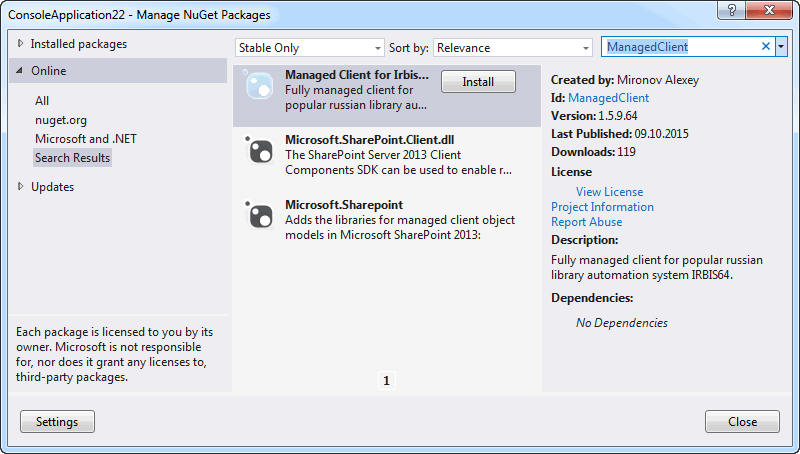
\includegraphics[width=0.7\textwidth]{nuget}
	\caption{Подключение библиотеки через NuGet}
\end{figure}


\begin{lstlisting}
using System;
using System.Linq;

using ManagedIrbis;

class Program
{
  private static void Main()
  {
    try
    {
      using (IrbisConnection connection = new IrbisConnection())
      {
        connection.ParseConnectionString
          (
            "host=127.0.0.1;port=6666;user=1;password=1;"
          );
        connection.Connect();

        int[] foundRecords = connection.Search
          (
            "\"A={0}$\"",
            "А"
          );

        int recordsToShow = Math.Min(foundRecords.Length, 10);

        for (int i = 0; i < recordsToShow; i++)
        {
          int thisMfn = foundRecords[i];

          MarcRecord record = connection.ReadRecord(thisMfn);

          string mainTitle = record
            .Fields
            .GetField("200")
            .GetSubField('a')
            .GetSubFieldText()
            .FirstOrDefault();

          Console.WriteLine
            (
              "MFN={0}, Main title={1}",
              thisMfn,
              mainTitle
            );

          Console.WriteLine
            (
              "BRIEF: {0}",
              client.FormatRecord("@brief", record)
            );

          MarcRecord newRecord = new MarcRecord();
          newRecord.AddField
            (
              "700",
              'a',
              "Управляемый клиент ИРБИС64"
            )
            .AddField
            (
              "200",
              'a', 
              string.Format ("Новая Запись от {0}", DateTime.Now),
              'f',
              "Управляемый клиент"
            );

          connection.WriteRecord
            (
              newRecord, 
              false, 
              true
            );

          Console.WriteLine(new string('-', 60));
        }
      }
    }
    catch (Exception ex)
    {
      Console.WriteLine(ex);
    }
  }
}\end{lstlisting}

\chapter*{Библиотека AM.Core}
\addcontentsline{toc}{chapter}{Библиотека AM.Core}

\backmatter
% bibliography, glossary and index would go here.

\listoffigures
\addcontentsline{toc}{chapter}{Список иллюстраций}
\listoftables
\addcontentsline{toc}{chapter}{Список таблиц}

\end{document}